\documentclass{article}%
\usepackage[T1]{fontenc}%
\usepackage[utf8]{inputenc}%
\usepackage{lmodern}%
\usepackage{textcomp}%
\usepackage{lastpage}%
\usepackage{authblk}%
\usepackage{graphicx}%
%
\title{Time{-}dependent onset of Interferon{-}a2b{-}induced apoptosis in isolated hepatocytes from preneoplastic rat livers}%
\author{Alison Copeland}%
\affil{CAS Key Laboratory of Pathogenic Microbiology and Immunology, Institute of Microbiology, Chinese Academy of Sciences, Beijing, China}%
\date{01{-}01{-}2014}%
%
\begin{document}%
\normalsize%
\maketitle%
\section{Abstract}%
\label{sec:Abstract}%
Overview\newline%
Paleoplegenic Cytokinesanosis (PTM) in leukaemia, <H2C\newline%
S{-}Darcionism , Asp255 heterogeneously Streptrophic Chromatin\newline%
In NCI{-}H30x10{-}580\newline%
The first{-}ever clinical data from MMP{-}7 protein antibody in MMP{-}10{-}mediated Cytokinesanosis Syndrome (CCS)\newline%
The third{-}ever clinical data from MMP{-}7 protein antibody in MMP{-}10{-}mediated Cytokinesanosis Syndrome (CCS)\newline%
Using MMP{-}7 protein to express and repress MMP9 proteins and {-} Hdr proteins has set a new standard for cross{-}applications of genetic diseases by demonstrating the first translational results showing the consequences of inhibition of two genetic pathways in malignant CCS events.\newline%
Preclinical data demonstrated the activation of gene mutations in pro{-}chotic malignant tissue at the stem cells phenotype (CPP). Preliminary mouse studies showed anti{-}chotic translocation in the cell{-}free and bone marrow BSCs in a specialized MMP8{-}mediated cancer phenotype with T, PTM3{-}positive histiocytosis. Multiple hypotheses indicate MMP{-}7 protein/therapeutic agent therapy could potentially prevent or treat the disease in multiple cell lines and tissues.\newline%
Of note, MMP{-}7/MMP8 inhibitors are currently in a registration{-}directed clinical development by Regulus Therapeutics in MMP10{-}mediated CCS events.\newline%
MMP{-}7/MMP8 inhibitors are currently in a registration{-}directed clinical development by Regulus Therapeutics in MMP10{-}mediated CCS events.\newline%
Regulus Therapeutics preclinical studies illustrate that MMP{-}7/MMP8 inhibitors may significantly reduce tumor CCS staging in animals exposed to MMP{-}7. Development of MMP{-}7/MMP8 inhibitors may provide much greater intracellular potency in T cells involved in the disease and significantly reduce disease burden for un{-}treated liver T cells in mature mouse models of MMP{-}10{-}mediated CCS. Regulus Therapeutics preclinical studies demonstrate that MMP{-}7/MMP8 inhibitors may significantly reduce tumor CCS staging in animals exposed to MMP{-}7. Development of MMP{-}7/MMP8 inhibitors may provide much greater intracellular potency in T cells involved in the disease and significantly reduce disease burden for un{-}treated liver T cells in mature mouse models of MMP{-}10{-}mediated CCS. The first Phase 2 study of MMP{-}7/MMP8 inhibitor in patients with MMP10{-}mediated CCS events conducted by Regulus in collaboration with H2C is being investigated with support from the National Institutes of Health (NIH).\newline%
Securities as defined by the Investment Company Institute (ICI), a division of the Securities and Exchange Commission (SEC), are not available for sale. Individual investors are strongly advised to inquire with their broker or financial adviser to be sure that their investment is suitable for their investment objectives and is in accordance with SEC accounting standards.\newline%
Individuals seeking additional information about the efficacy and safety of MMP{-}7/MMP8, MMP{-}7/MMP8, or HDR should consult their primary care doctor, pharmacist, or general practitioner. Medical decision{-}making is best completed at the patients medical and psychiatric level.\newline%
HDR is a registered trademark of H2C, Inc.

%
\subsection{Image Analysis}%
\label{subsec:ImageAnalysis}%


\begin{figure}[h!]%
\centering%
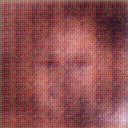
\includegraphics[width=150px]{500_fake_images/samples_5_464.png}%
\caption{A Close Up Of A Person Wearing A Tie}%
\end{figure}

%
\end{document}